% Requires: \usepackage{tikz, booktabs}

\begin{table}[htbp]
\centering
\caption{Truth tables for \texttt{sparse-dots} (run 0). Approaches disagree on 30/32 inputs.}
\label{tab:truth-table-sparse-dots}
\vspace{6pt}
\small
\begin{tabular}{c @{\hskip 12pt} c @{\hskip 12pt} c @{\hskip 12pt} c}
\toprule
Neighborhood & PCA & NCA & HyCA \\
\midrule
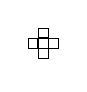
\begin{tikzpicture}[baseline=-0.5ex, scale=0.55] \fill[white, draw=black, line width=0.2pt] (0.24,0.48) rectangle ++(0.22,0.22); \fill[white, draw=black, line width=0.2pt] (0,0.24) rectangle ++(0.22,0.22); \fill[white, draw=black, line width=0.2pt] (0.24,0.24) rectangle ++(0.22,0.22); \fill[white, draw=black, line width=0.2pt] (0.48,0.24) rectangle ++(0.22,0.22); \fill[white, draw=black, line width=0.2pt] (0.24,0) rectangle ++(0.22,0.22); \end{tikzpicture} & 1 & 0 & 0 \\
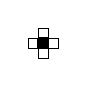
\begin{tikzpicture}[baseline=-0.5ex, scale=0.55] \fill[white, draw=black, line width=0.2pt] (0.24,0.48) rectangle ++(0.22,0.22); \fill[white, draw=black, line width=0.2pt] (0,0.24) rectangle ++(0.22,0.22); \fill[black, draw=black, line width=0.2pt] (0.24,0.24) rectangle ++(0.22,0.22); \fill[white, draw=black, line width=0.2pt] (0.48,0.24) rectangle ++(0.22,0.22); \fill[white, draw=black, line width=0.2pt] (0.24,0) rectangle ++(0.22,0.22); \end{tikzpicture} & 1 & 0 & 0 \\
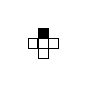
\begin{tikzpicture}[baseline=-0.5ex, scale=0.55] \fill[black, draw=black, line width=0.2pt] (0.24,0.48) rectangle ++(0.22,0.22); \fill[white, draw=black, line width=0.2pt] (0,0.24) rectangle ++(0.22,0.22); \fill[white, draw=black, line width=0.2pt] (0.24,0.24) rectangle ++(0.22,0.22); \fill[white, draw=black, line width=0.2pt] (0.48,0.24) rectangle ++(0.22,0.22); \fill[white, draw=black, line width=0.2pt] (0.24,0) rectangle ++(0.22,0.22); \end{tikzpicture} & 1 & 1 & 1 \\
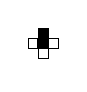
\begin{tikzpicture}[baseline=-0.5ex, scale=0.55] \fill[black, draw=black, line width=0.2pt] (0.24,0.48) rectangle ++(0.22,0.22); \fill[white, draw=black, line width=0.2pt] (0,0.24) rectangle ++(0.22,0.22); \fill[black, draw=black, line width=0.2pt] (0.24,0.24) rectangle ++(0.22,0.22); \fill[white, draw=black, line width=0.2pt] (0.48,0.24) rectangle ++(0.22,0.22); \fill[white, draw=black, line width=0.2pt] (0.24,0) rectangle ++(0.22,0.22); \end{tikzpicture} & 1 & 1 & 1 \\
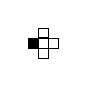
\begin{tikzpicture}[baseline=-0.5ex, scale=0.55] \fill[white, draw=black, line width=0.2pt] (0.24,0.48) rectangle ++(0.22,0.22); \fill[black, draw=black, line width=0.2pt] (0,0.24) rectangle ++(0.22,0.22); \fill[white, draw=black, line width=0.2pt] (0.24,0.24) rectangle ++(0.22,0.22); \fill[white, draw=black, line width=0.2pt] (0.48,0.24) rectangle ++(0.22,0.22); \fill[white, draw=black, line width=0.2pt] (0.24,0) rectangle ++(0.22,0.22); \end{tikzpicture} & 0 & 1 & 1 \\
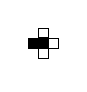
\begin{tikzpicture}[baseline=-0.5ex, scale=0.55] \fill[white, draw=black, line width=0.2pt] (0.24,0.48) rectangle ++(0.22,0.22); \fill[black, draw=black, line width=0.2pt] (0,0.24) rectangle ++(0.22,0.22); \fill[black, draw=black, line width=0.2pt] (0.24,0.24) rectangle ++(0.22,0.22); \fill[white, draw=black, line width=0.2pt] (0.48,0.24) rectangle ++(0.22,0.22); \fill[white, draw=black, line width=0.2pt] (0.24,0) rectangle ++(0.22,0.22); \end{tikzpicture} & 0 & 1 & 1 \\
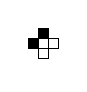
\begin{tikzpicture}[baseline=-0.5ex, scale=0.55] \fill[black, draw=black, line width=0.2pt] (0.24,0.48) rectangle ++(0.22,0.22); \fill[black, draw=black, line width=0.2pt] (0,0.24) rectangle ++(0.22,0.22); \fill[white, draw=black, line width=0.2pt] (0.24,0.24) rectangle ++(0.22,0.22); \fill[white, draw=black, line width=0.2pt] (0.48,0.24) rectangle ++(0.22,0.22); \fill[white, draw=black, line width=0.2pt] (0.24,0) rectangle ++(0.22,0.22); \end{tikzpicture} & 0 & 1 & 1 \\
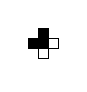
\begin{tikzpicture}[baseline=-0.5ex, scale=0.55] \fill[black, draw=black, line width=0.2pt] (0.24,0.48) rectangle ++(0.22,0.22); \fill[black, draw=black, line width=0.2pt] (0,0.24) rectangle ++(0.22,0.22); \fill[black, draw=black, line width=0.2pt] (0.24,0.24) rectangle ++(0.22,0.22); \fill[white, draw=black, line width=0.2pt] (0.48,0.24) rectangle ++(0.22,0.22); \fill[white, draw=black, line width=0.2pt] (0.24,0) rectangle ++(0.22,0.22); \end{tikzpicture} & 0 & 1 & 1 \\
\addlinespace[2pt]
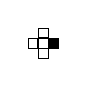
\begin{tikzpicture}[baseline=-0.5ex, scale=0.55] \fill[white, draw=black, line width=0.2pt] (0.24,0.48) rectangle ++(0.22,0.22); \fill[white, draw=black, line width=0.2pt] (0,0.24) rectangle ++(0.22,0.22); \fill[white, draw=black, line width=0.2pt] (0.24,0.24) rectangle ++(0.22,0.22); \fill[black, draw=black, line width=0.2pt] (0.48,0.24) rectangle ++(0.22,0.22); \fill[white, draw=black, line width=0.2pt] (0.24,0) rectangle ++(0.22,0.22); \end{tikzpicture} & 0 & 0 & 1 \\
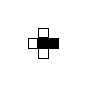
\begin{tikzpicture}[baseline=-0.5ex, scale=0.55] \fill[white, draw=black, line width=0.2pt] (0.24,0.48) rectangle ++(0.22,0.22); \fill[white, draw=black, line width=0.2pt] (0,0.24) rectangle ++(0.22,0.22); \fill[black, draw=black, line width=0.2pt] (0.24,0.24) rectangle ++(0.22,0.22); \fill[black, draw=black, line width=0.2pt] (0.48,0.24) rectangle ++(0.22,0.22); \fill[white, draw=black, line width=0.2pt] (0.24,0) rectangle ++(0.22,0.22); \end{tikzpicture} & 0 & 0 & 1 \\
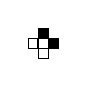
\begin{tikzpicture}[baseline=-0.5ex, scale=0.55] \fill[black, draw=black, line width=0.2pt] (0.24,0.48) rectangle ++(0.22,0.22); \fill[white, draw=black, line width=0.2pt] (0,0.24) rectangle ++(0.22,0.22); \fill[white, draw=black, line width=0.2pt] (0.24,0.24) rectangle ++(0.22,0.22); \fill[black, draw=black, line width=0.2pt] (0.48,0.24) rectangle ++(0.22,0.22); \fill[white, draw=black, line width=0.2pt] (0.24,0) rectangle ++(0.22,0.22); \end{tikzpicture} & 0 & 1 & 1 \\
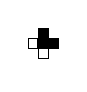
\begin{tikzpicture}[baseline=-0.5ex, scale=0.55] \fill[black, draw=black, line width=0.2pt] (0.24,0.48) rectangle ++(0.22,0.22); \fill[white, draw=black, line width=0.2pt] (0,0.24) rectangle ++(0.22,0.22); \fill[black, draw=black, line width=0.2pt] (0.24,0.24) rectangle ++(0.22,0.22); \fill[black, draw=black, line width=0.2pt] (0.48,0.24) rectangle ++(0.22,0.22); \fill[white, draw=black, line width=0.2pt] (0.24,0) rectangle ++(0.22,0.22); \end{tikzpicture} & 0 & 1 & 1 \\
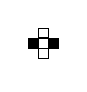
\begin{tikzpicture}[baseline=-0.5ex, scale=0.55] \fill[white, draw=black, line width=0.2pt] (0.24,0.48) rectangle ++(0.22,0.22); \fill[black, draw=black, line width=0.2pt] (0,0.24) rectangle ++(0.22,0.22); \fill[white, draw=black, line width=0.2pt] (0.24,0.24) rectangle ++(0.22,0.22); \fill[black, draw=black, line width=0.2pt] (0.48,0.24) rectangle ++(0.22,0.22); \fill[white, draw=black, line width=0.2pt] (0.24,0) rectangle ++(0.22,0.22); \end{tikzpicture} & 0 & 1 & 0 \\
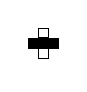
\begin{tikzpicture}[baseline=-0.5ex, scale=0.55] \fill[white, draw=black, line width=0.2pt] (0.24,0.48) rectangle ++(0.22,0.22); \fill[black, draw=black, line width=0.2pt] (0,0.24) rectangle ++(0.22,0.22); \fill[black, draw=black, line width=0.2pt] (0.24,0.24) rectangle ++(0.22,0.22); \fill[black, draw=black, line width=0.2pt] (0.48,0.24) rectangle ++(0.22,0.22); \fill[white, draw=black, line width=0.2pt] (0.24,0) rectangle ++(0.22,0.22); \end{tikzpicture} & 0 & 1 & 0 \\
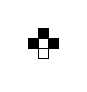
\begin{tikzpicture}[baseline=-0.5ex, scale=0.55] \fill[black, draw=black, line width=0.2pt] (0.24,0.48) rectangle ++(0.22,0.22); \fill[black, draw=black, line width=0.2pt] (0,0.24) rectangle ++(0.22,0.22); \fill[white, draw=black, line width=0.2pt] (0.24,0.24) rectangle ++(0.22,0.22); \fill[black, draw=black, line width=0.2pt] (0.48,0.24) rectangle ++(0.22,0.22); \fill[white, draw=black, line width=0.2pt] (0.24,0) rectangle ++(0.22,0.22); \end{tikzpicture} & 0 & 1 & 1 \\

\begin{tikzpicture}[baseline=-0.5ex, scale=0.55] \fill[black, draw=black, line width=0.2pt] (0.24,0.48) rectangle ++(0.22,0.22); \fill[black, draw=black, line width=0.2pt] (0,0.24) rectangle ++(0.22,0.22); \fill[black, draw=black, line width=0.2pt] (0.24,0.24) rectangle ++(0.22,0.22); \fill[black, draw=black, line width=0.2pt] (0.48,0.24) rectangle ++(0.22,0.22); \fill[white, draw=black, line width=0.2pt] (0.24,0) rectangle ++(0.22,0.22); \end{tikzpicture} & 0 & 1 & 1 \\
\addlinespace[2pt]
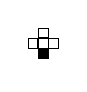
\begin{tikzpicture}[baseline=-0.5ex, scale=0.55] \fill[white, draw=black, line width=0.2pt] (0.24,0.48) rectangle ++(0.22,0.22); \fill[white, draw=black, line width=0.2pt] (0,0.24) rectangle ++(0.22,0.22); \fill[white, draw=black, line width=0.2pt] (0.24,0.24) rectangle ++(0.22,0.22); \fill[white, draw=black, line width=0.2pt] (0.48,0.24) rectangle ++(0.22,0.22); \fill[black, draw=black, line width=0.2pt] (0.24,0) rectangle ++(0.22,0.22); \end{tikzpicture} & 0 & 1 & 1 \\
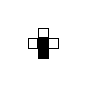
\begin{tikzpicture}[baseline=-0.5ex, scale=0.55] \fill[white, draw=black, line width=0.2pt] (0.24,0.48) rectangle ++(0.22,0.22); \fill[white, draw=black, line width=0.2pt] (0,0.24) rectangle ++(0.22,0.22); \fill[black, draw=black, line width=0.2pt] (0.24,0.24) rectangle ++(0.22,0.22); \fill[white, draw=black, line width=0.2pt] (0.48,0.24) rectangle ++(0.22,0.22); \fill[black, draw=black, line width=0.2pt] (0.24,0) rectangle ++(0.22,0.22); \end{tikzpicture} & 0 & 1 & 1 \\
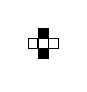
\begin{tikzpicture}[baseline=-0.5ex, scale=0.55] \fill[black, draw=black, line width=0.2pt] (0.24,0.48) rectangle ++(0.22,0.22); \fill[white, draw=black, line width=0.2pt] (0,0.24) rectangle ++(0.22,0.22); \fill[white, draw=black, line width=0.2pt] (0.24,0.24) rectangle ++(0.22,0.22); \fill[white, draw=black, line width=0.2pt] (0.48,0.24) rectangle ++(0.22,0.22); \fill[black, draw=black, line width=0.2pt] (0.24,0) rectangle ++(0.22,0.22); \end{tikzpicture} & 1 & 1 & 0 \\
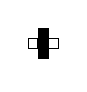
\begin{tikzpicture}[baseline=-0.5ex, scale=0.55] \fill[black, draw=black, line width=0.2pt] (0.24,0.48) rectangle ++(0.22,0.22); \fill[white, draw=black, line width=0.2pt] (0,0.24) rectangle ++(0.22,0.22); \fill[black, draw=black, line width=0.2pt] (0.24,0.24) rectangle ++(0.22,0.22); \fill[white, draw=black, line width=0.2pt] (0.48,0.24) rectangle ++(0.22,0.22); \fill[black, draw=black, line width=0.2pt] (0.24,0) rectangle ++(0.22,0.22); \end{tikzpicture} & 1 & 1 & 0 \\
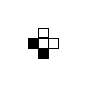
\begin{tikzpicture}[baseline=-0.5ex, scale=0.55] \fill[white, draw=black, line width=0.2pt] (0.24,0.48) rectangle ++(0.22,0.22); \fill[black, draw=black, line width=0.2pt] (0,0.24) rectangle ++(0.22,0.22); \fill[white, draw=black, line width=0.2pt] (0.24,0.24) rectangle ++(0.22,0.22); \fill[white, draw=black, line width=0.2pt] (0.48,0.24) rectangle ++(0.22,0.22); \fill[black, draw=black, line width=0.2pt] (0.24,0) rectangle ++(0.22,0.22); \end{tikzpicture} & 1 & 0 & 1 \\

\begin{tikzpicture}[baseline=-0.5ex, scale=0.55] \fill[white, draw=black, line width=0.2pt] (0.24,0.48) rectangle ++(0.22,0.22); \fill[black, draw=black, line width=0.2pt] (0,0.24) rectangle ++(0.22,0.22); \fill[black, draw=black, line width=0.2pt] (0.24,0.24) rectangle ++(0.22,0.22); \fill[white, draw=black, line width=0.2pt] (0.48,0.24) rectangle ++(0.22,0.22); \fill[black, draw=black, line width=0.2pt] (0.24,0) rectangle ++(0.22,0.22); \end{tikzpicture} & 1 & 0 & 1 \\
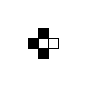
\begin{tikzpicture}[baseline=-0.5ex, scale=0.55] \fill[black, draw=black, line width=0.2pt] (0.24,0.48) rectangle ++(0.22,0.22); \fill[black, draw=black, line width=0.2pt] (0,0.24) rectangle ++(0.22,0.22); \fill[white, draw=black, line width=0.2pt] (0.24,0.24) rectangle ++(0.22,0.22); \fill[white, draw=black, line width=0.2pt] (0.48,0.24) rectangle ++(0.22,0.22); \fill[black, draw=black, line width=0.2pt] (0.24,0) rectangle ++(0.22,0.22); \end{tikzpicture} & 0 & 1 & 1 \\

\begin{tikzpicture}[baseline=-0.5ex, scale=0.55] \fill[black, draw=black, line width=0.2pt] (0.24,0.48) rectangle ++(0.22,0.22); \fill[black, draw=black, line width=0.2pt] (0,0.24) rectangle ++(0.22,0.22); \fill[black, draw=black, line width=0.2pt] (0.24,0.24) rectangle ++(0.22,0.22); \fill[white, draw=black, line width=0.2pt] (0.48,0.24) rectangle ++(0.22,0.22); \fill[black, draw=black, line width=0.2pt] (0.24,0) rectangle ++(0.22,0.22); \end{tikzpicture} & 0 & 1 & 1 \\
\addlinespace[2pt]
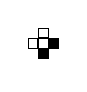
\begin{tikzpicture}[baseline=-0.5ex, scale=0.55] \fill[white, draw=black, line width=0.2pt] (0.24,0.48) rectangle ++(0.22,0.22); \fill[white, draw=black, line width=0.2pt] (0,0.24) rectangle ++(0.22,0.22); \fill[white, draw=black, line width=0.2pt] (0.24,0.24) rectangle ++(0.22,0.22); \fill[black, draw=black, line width=0.2pt] (0.48,0.24) rectangle ++(0.22,0.22); \fill[black, draw=black, line width=0.2pt] (0.24,0) rectangle ++(0.22,0.22); \end{tikzpicture} & 1 & 0 & 1 \\
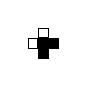
\begin{tikzpicture}[baseline=-0.5ex, scale=0.55] \fill[white, draw=black, line width=0.2pt] (0.24,0.48) rectangle ++(0.22,0.22); \fill[white, draw=black, line width=0.2pt] (0,0.24) rectangle ++(0.22,0.22); \fill[black, draw=black, line width=0.2pt] (0.24,0.24) rectangle ++(0.22,0.22); \fill[black, draw=black, line width=0.2pt] (0.48,0.24) rectangle ++(0.22,0.22); \fill[black, draw=black, line width=0.2pt] (0.24,0) rectangle ++(0.22,0.22); \end{tikzpicture} & 1 & 0 & 1 \\
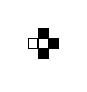
\begin{tikzpicture}[baseline=-0.5ex, scale=0.55] \fill[black, draw=black, line width=0.2pt] (0.24,0.48) rectangle ++(0.22,0.22); \fill[white, draw=black, line width=0.2pt] (0,0.24) rectangle ++(0.22,0.22); \fill[white, draw=black, line width=0.2pt] (0.24,0.24) rectangle ++(0.22,0.22); \fill[black, draw=black, line width=0.2pt] (0.48,0.24) rectangle ++(0.22,0.22); \fill[black, draw=black, line width=0.2pt] (0.24,0) rectangle ++(0.22,0.22); \end{tikzpicture} & 0 & 1 & 1 \\
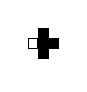
\begin{tikzpicture}[baseline=-0.5ex, scale=0.55] \fill[black, draw=black, line width=0.2pt] (0.24,0.48) rectangle ++(0.22,0.22); \fill[white, draw=black, line width=0.2pt] (0,0.24) rectangle ++(0.22,0.22); \fill[black, draw=black, line width=0.2pt] (0.24,0.24) rectangle ++(0.22,0.22); \fill[black, draw=black, line width=0.2pt] (0.48,0.24) rectangle ++(0.22,0.22); \fill[black, draw=black, line width=0.2pt] (0.24,0) rectangle ++(0.22,0.22); \end{tikzpicture} & 0 & 1 & 1 \\

\begin{tikzpicture}[baseline=-0.5ex, scale=0.55] \fill[white, draw=black, line width=0.2pt] (0.24,0.48) rectangle ++(0.22,0.22); \fill[black, draw=black, line width=0.2pt] (0,0.24) rectangle ++(0.22,0.22); \fill[white, draw=black, line width=0.2pt] (0.24,0.24) rectangle ++(0.22,0.22); \fill[black, draw=black, line width=0.2pt] (0.48,0.24) rectangle ++(0.22,0.22); \fill[black, draw=black, line width=0.2pt] (0.24,0) rectangle ++(0.22,0.22); \end{tikzpicture} & 1 & 0 & 1 \\

\begin{tikzpicture}[baseline=-0.5ex, scale=0.55] \fill[white, draw=black, line width=0.2pt] (0.24,0.48) rectangle ++(0.22,0.22); \fill[black, draw=black, line width=0.2pt] (0,0.24) rectangle ++(0.22,0.22); \fill[black, draw=black, line width=0.2pt] (0.24,0.24) rectangle ++(0.22,0.22); \fill[black, draw=black, line width=0.2pt] (0.48,0.24) rectangle ++(0.22,0.22); \fill[black, draw=black, line width=0.2pt] (0.24,0) rectangle ++(0.22,0.22); \end{tikzpicture} & 1 & 0 & 1 \\

\begin{tikzpicture}[baseline=-0.5ex, scale=0.55] \fill[black, draw=black, line width=0.2pt] (0.24,0.48) rectangle ++(0.22,0.22); \fill[black, draw=black, line width=0.2pt] (0,0.24) rectangle ++(0.22,0.22); \fill[white, draw=black, line width=0.2pt] (0.24,0.24) rectangle ++(0.22,0.22); \fill[black, draw=black, line width=0.2pt] (0.48,0.24) rectangle ++(0.22,0.22); \fill[black, draw=black, line width=0.2pt] (0.24,0) rectangle ++(0.22,0.22); \end{tikzpicture} & 0 & 1 & 0 \\

\begin{tikzpicture}[baseline=-0.5ex, scale=0.55] \fill[black, draw=black, line width=0.2pt] (0.24,0.48) rectangle ++(0.22,0.22); \fill[black, draw=black, line width=0.2pt] (0,0.24) rectangle ++(0.22,0.22); \fill[black, draw=black, line width=0.2pt] (0.24,0.24) rectangle ++(0.22,0.22); \fill[black, draw=black, line width=0.2pt] (0.48,0.24) rectangle ++(0.22,0.22); \fill[black, draw=black, line width=0.2pt] (0.24,0) rectangle ++(0.22,0.22); \end{tikzpicture} & 0 & 1 & 0 \\
\bottomrule
\end{tabular}
\end{table}